\documentclass[a4paper,12pt]{report}
\usepackage{amsmath,amsthm,amssymb,graphicx,float,tikz,tkz-euclide,geometry,hyperref}

\hypersetup{hidelinks}

\hyphenpenalty=10000

\newtheorem*{theorem}{Theorem}
\newtheorem*{prop}{Proposition}
\newtheorem*{lemma}{Lemma}

\theoremstyle{definition}
\newtheorem*{definition}{Definition}
\newtheorem*{ex}{Ex}

\theoremstyle{remark}
\newtheorem*{remark}{Remark}

\renewcommand\qedsymbol{$\blacksquare$}

\newcommand{\R}{\mathbb{R}}
\newcommand{\Q}{\mathbb{Q}}
\newcommand{\Z}{\mathbb{Z}}
\newcommand{\C}{\mathbb{C}}
\newcommand{\N}{\mathbb{N}}
\newcommand{\F}{\mathbb{F}}

\addtocontents{toc}{\protect\setcounter{tocdepth}{1}}

\begin{document}
  \title{\Huge\textbf{Projective Geometry}}
  \author{Tejaswi\\[1cm]{\small Advisor: Dr. Steven Spallone}}
  \date{Summer 2025}
  \maketitle

  \pagenumbering{roman}

  \tableofcontents
  \newpage

  \pagenumbering{arabic}

  \chapter{Basic Algebra}
\label{chap:basics}

\section{Groups, Rings and Fields}

\subsection{Groups}

\begin{definition}
  A \textit{group} is an ordered pair $(G,\ast)$ where $G$ is a set and $\ast$ is a binary
  operation on $G$ satisfying the following axioms:

  \begin{itemize}
    \item[(i)] $(a\ast b)\ast c=a\ast(b\ast c)\forall a,b\in G$,
    \item[(ii)] $\exists e\in G$, called identity of $G$, such that $\forall a\in G$ we have 
      $a\ast e=e\ast a=a$,
    \item[(iii)] for each $a\in G$, $\exists a^{-1}\in G$, called inverse of $a$, such that 
      $a\ast a^{-1}=a^{-1}\ast a=e$,
  \end{itemize}

  The group is called abelian is $a\ast b=b\ast a\forall a,b\in G$. \cite{dummit}
\end{definition}

\begin{ex}
  $\Z$, $\Q$, $\R$, and $\C$ are groups under $+$ with $e=0$, and $a^{-1}=-a$ for all $a$, and
  $\Q-\{0\}$, $\R-\{0\}$, and $\C-\{0\}$ are groups under $\times$ with $e=1$ and
  $a^{-1}=\frac{1}{a}$ for all $a$.
\end{ex}

\begin{remark}
  If $G$ is a group under the opertaion $\ast$, then

  \begin{enumerate}
    \item the identity of $G$ is unique,
    \item for each $a\in G$, $a^{-1}$ is uniquely determined,
    \item $(a^{-1})^{-1}=a$ for all $a\in G$,
    \item $(a\ast b)^{-1}=b^{-1}\ast a^{-1}$,
    \item for any $a_1,a_2,\ldots,a_n\in G$, the value of $a_1\ast a_2\ast\ldots\ast a_n$ is
        independent of how the expression is bracketed,
    \item if $a\ast u=a\ast v$, then $u=v$, and if $u\ast b=v\ast b$, then $u=v$.
  \end{enumerate}

\end{remark}

\begin{definition}
  Let $(G,\ast)$ and $(H,\diamond)$ be groups. A map $\phi:G\rightarrow H$ such that
  $\phi(x\ast y)=\phi(x)\diamond\phi(y)$ for all $x,y\in G$ is called a \textit{homomorphism}.
  The map is called an \textit{isomorphism} and $G$ and $H$ are said to be \textit{isomorphic},
  written $G\cong H$, if $\phi$ is a bijective homomorphism. \cite{dummit}
\end{definition}

\begin{ex}
  For any group $G$, $G\cong G$. The identity map provides an obviuos isomorphism.\\
  - The exponentiation map $exp:\R\rightarrow \R^+$ defined by $exp(x)=e^x$, is an isomorphism
  from $(\R,+)$ to $(\R^+,\times)$.
\end{ex}

\subsection{Fields}

\begin{definition}
  A \textit{field} is a set $F$ together with two binary operations $+$ and $\times$ such that
  $(F,+)$ is an abelian group and $(F-\{0\},\times)$ is also an an abelian group, and the
  following distribution law holds: $a\times(b+c)=(a\times b)+(a\times c)$ for all $a,b,c\in F$.
  \cite{dummit}
\end{definition}

\begin{ex}
  With usual addition and multiplication, $\Q$ and $\R$ are fields.\\
   - $\Z/p\Z$, where $p$ is a prime, with modular addition and multiplication, is a finite
  field.
\end{ex}

\begin{remark}
  For any field $F$ if $\vert F\vert <\infty$, then $\vert F\vert = p^m$ for some prime $p$
  and some interger $m$.
\end{remark}

\begin{definition}
  The \textit{charfecteristic} of a field $F$, denoted by $ch(F)$, is defined to be the smallest
  positive integer $p$ such that $p\cdot 1_F=0$ if such $p$ exists, and defined to be zero
  otherwise. \cite{dummit}
\end{definition}

\begin{remark}
  The charecteristic of a field $F$, $ch(F)$, is either $0$ or a prime $p$.
\end{remark}

\subsection{Rings}

\begin{definition}
  A \textit{ring} $R$ is a set together with two binary operations $+$ and $\times$ satisfying
  the following axioms

  \begin{itemize}
    \item[(i)] $(R,+)$ is an abelian group,
    \item[(ii)] $\times$ is associative: $(a\times b)\times c=a\times(b\times c)$ for all $a,b,c\in R$,
    \item[(iii)] the distributive laws hold in $R$: for all $a,b,c\in R$,
        $(a+b)\times c=(a\times c)+(b\times c)$ and $a\times(b+c)=(a\times b)+(a\times c)$
  \end{itemize}

  The ring $R$ is coommutative if $R$ is commutative. $R$ is said to have an identity if there
  is an element $1\in R$ with $1\times a=a\times 1$ for all $a\in R$. \cite{dummit}
\end{definition}

\begin{ex}
  All fields are obviously rings.\\
   - The simplest rings are \textit{trivial rings}, obtained by taking $R$ to be any abelian
  group and defining multiplication $\times$ on $R$ by $a\times b=0$ for all $(a,b)\in R$.
  \textit{trivial rings} are also commutative, as obviuos from the definition.\\
   - The ring of integers $\Z$ - under usual addition and multiplication is a commutative ring
  with identity $1$.
\end{ex}

\section{Field Extensions}

\begin{definition}
  If $K$ is a field containing the subfield $F$, then $K$ is said to be an \textit{extension} of
  $F$, denoted $K/F$. The field $F$ is sometimes called the base field of the extension.
  \cite{dummit}
\end{definition}

\begin{definition}
  The \textit{prime subfield} of a field $F$ is the subfield of $F$ generated by its
  multiplicative identity $1_F$. It is isomorphic to either $\Q$(if $ch(F)=0$), or to
  $\F_p$(if $ch(F)=p$). \cite{dummit}
\end{definition}

\begin{remark}
  Every field $F$ is an extension of its prime subfield.
\end{remark}

\begin{definition}
  The \textit{degree} of a field extension $K/F$, denoted $[K:F]$, is the dimension of $K$ as a
  vector space over $F$. \cite{dummit}
\end{definition}

An important class of field extensions are those obtained by trying to solve equations over
a field $F$. Famously, Gauss extended $\R$ in an attempt to solve the equation $x^2+1=0$.
The new field generated by adjoining the roots of the equation $i$ and $-i$ to $\R$ is $\C$.
Given any field $F$ and a polynomial $p(x)\in F[x]$, one can similarly extend it to form a field
$K$, containing solution to the equation $p(x)=0$.

  \chapter{Conics} \label{ch:conics}

The majority of this chapter is based on the ideas presented in Shirali's article
on conic groups \cite{shirali}. We'll also develop this further with the chapter
on conics over characteristic two fields.

\section{Group Laws on Conics}

Consider a non-degenerate conic section $\mathcal{C}$ and a point $O \in
\mathcal{C}$. For any points $P,Q\in\mathcal{C}$, let $\ell'$ be the line passing
through $O$ such that $\ell' \parallel \ell$ where $\ell$ is the line joining $P$
and $Q$. If $\ell'$ intersects $\mathcal{C}$ at a point other than $O$, call that
point $R$. Otherwise, take $R=O$. Define a binary operation
$\conop : \mathcal{C} \times \mathcal{C} \to \mathcal{C}$ as $P \conop Q := R$.
\vspace{1ex}

\begin{figure}[H]
    \center
    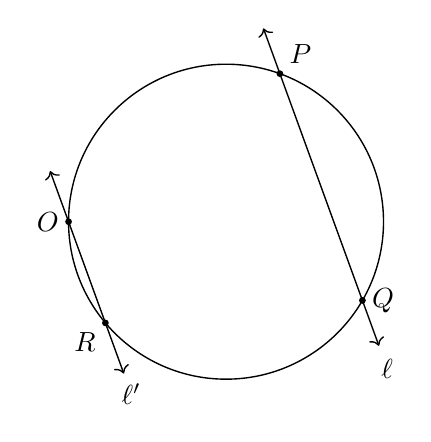
\begin{tikzpicture}
        \tkzDefPoint(0,0){C}
        \tkzDefPoint(-2,0){O}
        \tkzDefPoint({2*cos(70*pi/180)},{2*sin(70*pi/180)}){P}
        \tkzDefPoint({2*cos(-30*pi/180)},{2*sin(-30*pi/180)}){Q}
        \tkzDefPoint({2*cos(-140*pi/180)},{2*sin(-140*pi/180)}){R}

        \tkzDrawPoints[fill=black](O,P,Q,R)
        \tkzDrawLine[<->,line width=0.5,add=0.2 and 0.2](P,Q)
        \tkzDrawLine[<->,line width=0.5,add=0.5 and 0.5](O,R)
        \tkzDrawCircle[color=black,line width=0.5](C,O)

        \tkzLabelPoints[left](O)
        \tkzLabelPoints[above right](P)
        \tkzLabelPoints[right](Q)
        \tkzLabelPoints[below left](R)

        \tkzLabelLine[pos=1.3](P,Q){$\ell$}
        \tkzLabelLine[pos=1.7](O,R){$\ell'$}
    \end{tikzpicture}

    \caption{$P \conop Q$ when $\mathcal{C}$ is a circle.}
\end{figure}

We'll first find formulae to calculate $P \conop Q$ and then proceed to prove
that $\mathcal{C}$ is a group with $\conop$.
\subsection*{A Note on Standard Forms}

Throughout this section, we'll only use standard forms of non-degenerate conics
i.e. circle, rectangular hyperbola and parabola with equations $x^2+y^2=1$, $xy=1$
and $y=x^2$ respectively. In the next chapter, we'll show that any ellipse,
hyperbola and parabola is affine-congruent to these standard forms; generalizing
our results to all conics.

\subsection*{Circle}

If $\mathcal{C}=\mathcal{S}$ with equation $x^2+y^2=1$, any point
$P\in\mathcal{S}$ has coordinates $(\cos t,\sin t)$ where $t\in[0,2\pi)$ is the
angle $P$ forms with the positive $x$-axis in the counter-clockwise direction.
\vspace{1ex}

Let $O,P,Q,R\in\mathcal{P}$ be points with parameters $t_0$, $t_1$, $t_2$ and
$t_3$ respectively such that $P \conop Q = R$. By definition of $P \conop Q$, we
have $PQ \parallel OR$. Note that if $P=Q$, then slope at $P$ is
\[
    y'|_{x=t_1} = \left(-\frac{x}{y}\right)_{t=t_1}
    = \left(-\frac{\cos t}{\sin t}\right)_{t=t_1}
                = -\cot t_1
                = -\cot \left(\frac{t_1+t_2}{2}\right)
\]
and if $P \neq Q$, then $t_1 \neq t_2$ and slope of $PQ$ is 
\[
    \frac{\sin t_2 - \sin t_1}{\cos t_2 - \cos t_1}
    = -\frac{\sin\left(\frac{t_2-t_1}{2}\right)\cos\left(\frac{t_2+t_1}{2}\right)}{\sin\left(\frac{t_2-t_1}{2}\right)\sin\left(\frac{t_2+t_1}{2}\right)}
    = -\cot\left(\frac{t_2+t_1}{2}\right)
\]
Also note that $\sin\left(\frac{t_2 - t_1}{2}\right)$ can be cancelled as it's
only zero when $t_2=t_1+2n\pi$ which means $P=Q$. So, we don't need to consider
the points being same as a separate case. Equating slopes of $PQ$ and $OR$, we
get,
\begin{align*}
    &-\cot\left(\frac{t_2+t_1}{2}\right) = -\cot\left(\frac{t_3+t_0}{2}\right) \\
    \implies& \frac{t_2+t_1}{2} = n\pi+\frac{t_3+t_0}{2} \\
    \implies& t_3 = t_2 + t_1 - t_0 - 2n\pi
\end{align*}

\noindent
As shifts of $2n\pi$ don't affect $t_3$, we can ignore that term on the RHS.
Thus for any $P,Q\in\mathcal{S}$ with parameters $t_1$ and $t_2$
respectively for circle $\mathcal{S}$, $P \conop Q = R$ has parameter
$t_3 = t_1 + t_2 - t_0$ where $t_0$ is the parameter for point
$O$. Note that we always add or subtract multiples of $2\pi$ to make sure
$t_3\in[0,2\pi)$.
\vspace{1ex}

It is easy to see that $\conop$ satisfies closure for $\mathcal{S}$. We'll verfiy each of 
the group axioms now.

\begin{enumerate}
    \item{\textbf{Identity:}} For any $P \in \mathcal{S}$ with parameter $t$,
        $P \conop O$ will have parameter
        \[ t' = t + t_0 - t_0 = t \]
        Thus $O$ acts as the identity element for $\conop$.

    \item{\textbf{Inverse:}} The point $Q\in\mathcal{S}$ with parameter
        $2t_0 - t$ gives the parameter of $P \conop Q$ to be
        \[ t' = t + 2t_0 - t - t_0 = t_0 \]
        Hence, $Q$ is the inverse of $P$.

    \item{\textbf{Associativity:}} For any $P,Q,R \in \mathcal{S}$ with parameters\
        $t_1$, $t_2$ and $t_3$ respectively, $P\conop(Q \conop R)$
        has parameter
        \[
            t_1 + (t_2 + t_3 - t_0) - t_0 =
            t_1 + t_2 + t_3 - 2t_0
        \]
        On the other hand, $(P \conop Q)\conop R$ has parameter
        \[
            (t_1 + t_2 - t_0) + t_3 - t_0 =
            t_1 + t_2 + t_3 - 2t_0
        \]
        Thus $\conop$ is associative.
\end{enumerate}

\noindent
This shows that $\mathcal{S}$ is a group with $\conop$.

\begin{theorem}
    $\langle \mathcal{S},\conop \rangle \cong \langle S^1,\cdot \rangle$ where
    $S^1=\{e^{i\theta}\in\mathbb{C}: \theta \in [0,2\pi)\}$.
\end{theorem}

\begin{proof}
    Consider $\varphi:\mathcal{S} \to S^1$ given by
    $\varphi((\cos\theta,\sin\theta)) = e^{i(\theta-\theta_0)}$. For any points
    $P,Q\in\mathcal{S}$ parametrized by $\theta_1$ and $\theta_2$ respectively,
    $P \conop Q$ has parameter $\theta_1 + \theta_2 - \theta_0$. So,
    \[
        \varphi(P \conop Q) = e^{i(\theta_1 + \theta_2 - 2\theta_0)}
        = e^{i(\theta_1 - \theta_0)}e^{i(\theta_2 - \theta_0)} = \varphi(P)\varphi(Q)
    \]
    Thus $\varphi$ is a homomorphism.
    \vspace{1ex}

    \noindent
    If $\varphi(P)=\varphi(Q)$ for some $P,Q\in\mathcal{S}$ parametrized by
    $\theta_1$ and $\theta_2$ respectively, then
    \begin{align*}
        e^{i(\theta_1-\theta_0)} = e^{i(\theta_2-\theta_0)}
        \implies e^{i\theta_1}e^{-i\theta_0} = e^{i\theta_2}e^{-i\theta_0}
        \implies e^{i\theta_1} = e^{i\theta_2}
        \implies \theta_1 = 2n\pi + \theta_2
    \end{align*}
    i.e. $P=Q$. Thus $\varphi$ is injective.
    \vspace{1ex}

    \noindent
    For any $e^{i\theta} \in S^1$, we have the point
    $P=(\cos(\theta+\theta_0),\sin(\theta+\theta_0)) \in \mathcal{S}$ such that
    \[ \varphi(P) = e^{i(\theta + \theta_0 - \theta_0)} = e^{i\theta} \]
    Thus $\varphi$ is surjective. This shows that $\varphi$ is a bijective
    homomorphism i.e. an isomorphism from $\langle \mathcal{S},\conop \rangle$ to
    $\langle S^1,\cdot \rangle$.
\end{proof}

\subsection*{Parabola}

If $\mathcal{C}=\mathcal{P}$ is the parabola with equation $y=x^2$, any point on
it can be parametrized as $(t,t^2)$ where $t\in\mathbb{R}$.
\vspace{1ex}

Let $O,P,Q,R\in\mathcal{P}$ be points with parameters $t_0$, $t_1$, $t_2$ and
$t_3$ respectively such that $P \conop Q = R$. By definition of $P \conop Q$, we
have $PQ \parallel OR$. Note that if $P=Q$, then slope at $P$ is
\[
    y'|_{x=t_1} = \left(2x\right)_{x=t_1} = 2t_1 = t_1 + t_2
\]
and if $P \neq Q$, then $t_1 \neq t_2$ and slope of $PQ$ is 
\[
    \frac{t_2^2-t_1^2}{t_2-t_1} = t_1 + t_2
\]
So, we don't need to consider the points being same as a separate case. Equating
slopes of $PQ$ and $OR$, we get,
\[ t_1 + t_2 = t_0 + t_3 \implies t_3 = t_1 + t_2 - t_0 \]

Thus, for any points $P,Q\in\mathcal{P}$ with parameters $t_1$ and $t_2$
respectively for a parabola $\mathcal{P}$, $P \conop Q = R$ has parameter
$t_3 = t_1 + t_2 - t_0$ where $t_0$ is the parameter for point $O$.
\vspace{1ex}

It is easy to see that $\conop$ satisfies closure for $\mathcal{P}$. We'll verfiy
each of the group axioms now.

\begin{enumerate}
    \item{\textbf{Identity:}} For any $P\in\mathcal{P}$ with parameter $t$,
        $P \conop O$ will have parameter
        \[ t' = t + t_0 - t_0 = t \]
        Thus $O$ acts as the identity element for $\conop$.

    \item{\textbf{Inverse:}} The point $Q\in\mathcal{P}$ with parameter $2t_0 - t$
        gives the parameter of $P \conop Q$ to be
        \[ t' = t + 2t_0 - t - t_0 = t_0 \]
        Hence, $Q$ is the inverse of $P$.

    \item{\textbf{Associativity:}} For any $P,Q,R \in \mathcal{P}$ with parameters
        $t_1$, $t_2$ and $t_3$ respectively, $P\conop(Q \conop R)$ has parameter
        \[ t_1 + (t_2 + t_3 - t_0) - t_0 = t_1 + t_2 + t_3 - 2t_0 \]
        On the other hand, $(P \conop Q)\conop R$ has parameter
        \[ (t_1 + t_2 - t_0) + t_3 - t_0 = t_1 + t_2 + t_3 - 2t_0 \]
        Thus $\conop$ is associative.
\end{enumerate}

\noindent
This shows that $\mathcal{P}$ is a group with $\conop$.

\begin{theorem}
    $\langle \mathcal{P},\conop \rangle \cong \langle \mathbb{R},+ \rangle$.
\end{theorem}

\begin{proof}
    Consider $\varphi:\mathcal{P} \to \mathbb{R}$ given by
    $\varphi((t,t^2)) = t - t_0$. For any points
    $P,Q\in\mathcal{P}$ parametrized by $t_1$ and $t_2$ respectively,
    $P \conop Q$ has parameter $t_1 + t_2 - t_0$. So,
    \[
        \varphi(P \conop Q) = t_1 + t_2 - 2t_0 = (t_1 - t_0) + (t_2 - t_0)
        = \varphi(P) + \varphi(Q)
    \]
    Thus $\varphi$ is a homomorphism.
    \vspace{1ex}

    \noindent
    If $\varphi(P)=\varphi(Q)$ for some $P,Q\in\mathcal{P}$ parametrized by $t_1$
    and $t_2$ respectively, then
    \begin{align*}
        t_1 - t_0 = t_2 - t_0 \implies t_1 = t_2
    \end{align*}
    i.e. $P=Q$. Thus $\varphi$ is injective.
    \vspace{1ex}

    \noindent
    For any $t \in \mathbb{R}$, we have the point
    $P=(t + t_0,(t + t_0)^2) \in \mathcal{P}$ such that
    \[ \varphi(P) = t + t_0 - t_0 = t \]
    Thus $\varphi$ is surjective. This shows that $\varphi$ is a bijective
    homomorphism i.e. an isomorphism from $\langle \mathcal{P},\conop \rangle$ to
    $\langle \mathbb{R},+ \rangle$.
\end{proof}

\subsection*{Hyperbola}

If $\mathcal{C}=\mathcal{H}$ is the rectangular hyperbola with equation $xy=1$,
any point on it can be parametrized as $(t,t^{-1})$ where $t\in\mathbb{R}^\times$.
\vspace{1ex}

Let $O,P,Q,R\in\mathcal{H}$ be points with parameters $t_0$, $t_1$, $t_2$ and
$t_3$ respectively such that $P \conop Q = R$. By definition of $P \conop Q$, we
have $PQ \parallel OR$. Note that if $P=Q$, then slope at $P$ is
\[
    y'|_{x=t_1} = \left(-\frac{1}{x^2}\right)_{x=t_1}
    = -\frac{1}{t_1^2} = -\frac{1}{t_1 t_2}
\]
and if $P \neq Q$, then $t_1 \neq t_2$ and slope of $PQ$ is 
\[
    \frac{t_2^{-1}-t_1^{-1}}{t_2-t_1} = \frac{t_1 - t_2}{t_1 t_2 (t_2 - t_1)}
    = -\frac{1}{t_1 t_2}
\]
So, we don't need to consider points being same as a separate case. Equating
slopes of $PQ$ and $OR$, we get,
\[ -\frac{1}{t_1 t_2} = -\frac{1}{t_0 t_3} \implies t_3 = \frac{t_1 t_2}{t_0} \]

Thus, for any points $P,Q\in\mathcal{H}$ with parameters $t_1$ and $t_2$
respectively for a rectangular hyperbola $\mathcal{H}$, $P \conop Q = R$ has
parameter $t_3 = t_1 t_2 t_0^{-1}$ where $t_0$ is the parameter corresponding to
point $O$.
\vspace{1ex}

It is easy to see that $\conop$ satisfies closure for $\mathcal{H}$. We'll verfiy
each of  the group axioms now.

\begin{enumerate}
    \item{\textbf{Identity:}} For any $P\in\mathcal{H}$ with parameter $t$,
        $P \conop O$ will have parameter
        \[ t' = t t_0 t_0^{-1} = t \]
        Thus $O$ acts as the identity element for $\conop$.

    \item{\textbf{Inverse:}} The point $Q\in\mathcal{H}$ with parameter
        $t_0^2 t^{-1}$ gives the parameter of $P \conop Q$ to be
        \[ t' = t (t_0^2 t^{-1}) t_0^{-1} = t_0 \]
        Hence, $Q$ is the inverse of $P$.

    \item{\textbf{Associativity:}} For any $P,Q,R\in\mathcal{H}$ with parameters
        $t_1$, $t_2$ and $t_3$ respectively, $P\conop(Q \conop R)$ has parameter
        \[ t_1 (t_2 t_3 t_0^{-1}) t_0^{-1} = t_1 t_2 t_3 t_0^{-2} \]
        On the other hand, $(P \conop Q)\conop R$ has parameter
        \[ (t_1 t_2 t_0^{-1}) t_3 t_0^{-1} = t_1 t_2 t_3 t_0^{-2} \]
        Thus $\conop$ is associative.
\end{enumerate}

\noindent
This shows that $\mathcal{H}$ is a group with $\conop$.

\begin{theorem}
    $\langle \mathcal{H},\conop \rangle \cong \langle \mathbb{R}^\times,\cdot \rangle$.
\end{theorem}

\begin{proof}
    Consider $\varphi:\mathcal{H} \to \mathbb{R}^\times$ given by
    $\varphi((t,t^{-1})) = t t_0^{-1}$. For any points
    $P,Q\in\mathcal{H}$ parametrized by $t_1$ and $t_2$ respectively,
    $P \conop Q$ has parameter $t_1 t_2 t_0^{-1}$. So,
    \[
        \varphi(P \conop Q) = t_1 t_2 t_0^{-2} = (t_1 t_0^{-1}) (t_2 t_0^{-1})
        = \varphi(P) \varphi(Q)
    \]
    Thus $\varphi$ is a homomorphism.
    \vspace{1ex}

    \noindent
    If $\varphi(P)=\varphi(Q)$ for some $P,Q\in\mathcal{H}$ parametrized by $t_1$
    and $t_2$ respectively, then
    \begin{align*}
        t_1 t_0^{-1} = t_2 t_0^{-1} \implies t_1 = t_2
    \end{align*}
    i.e. $P=Q$. Thus $\varphi$ is injective.
    \vspace{1ex}

    \noindent
    For any $t \in \mathbb{R}$, we have the point
    $P=(t t_0,(t t_0)^{-1}) \in \mathcal{H}$ such that
    \[ \varphi(P) = t t_0 t_0^{-1} = t \]
    Thus $\varphi$ is surjective. This shows that $\varphi$ is a bijective
    homomorphism i.e. an isomorphism from $\langle \mathcal{H},\conop \rangle$ to
    $\langle \mathbb{R}^\times,\cdot \rangle$.
\end{proof}

\section{Generalizing to any field}

\paragraph{Note:} \emph{Throughout this section, we'll limit ourselves to fields
    whose characteristic is not 2 as fields with characteristic 2 require a more
    careful treatment. We'll have a look at these in Chapter \ref{ch:char2}.}
\vspace{1ex}

\noindent
In the previous section, we've considered our conic as the set of points
$(x,y)\in\mathbb{R}^2$ that make $f(x,y)=0$ where $f\in\mathbb{R}[x,y]$ is
square-free and has degree 2. We could very well have considered a similar set
for any field $\mathbb{F}$ and we'll
now show how a similar operation gives rise to a group structure.
\vspace{1ex}

\noindent
We'll consider $\mathbb{F}^2$ as a vector space for the rest of this section. 
Consider a set
\[ \mathcal{C} = \{(x,y)\in\mathbb{F}^2: f(x,y)=0\} \]
where $f\in\mathbb{F}[x,y]$ is square-free and has degree 2. Fix an
$\vec O=(x_0,y_0)\in\mathcal{C}$.  For any $\vec{A},\vec{B}\in\mathcal{C}$ where
$\vec{A}=(a_1,a_2)$ and $\vec{B}=(b_1,b_2)$.
\vspace{1ex}

\noindent
Let 
\begin{align*}
    \vec{c} &=
        \begin{cases}
            \vec{B}-\vec{A} & \mathrm{if}\ \vec{A}\neq\vec{B} \\
            \left(
                \frac{\partial f}{\partial y}, -\frac{\partial f}{\partial x}
            \right)_{(x,y)=\vec{A}} & \mathrm{otherwise}
        \end{cases} \\
    \ell &=
        \{\vec{x}\in\mathbb{F}^2:
        \vec{x} = \vec{O} + \lambda\vec{c}\quad\forall\lambda\in\mathbb{F}\}
\end{align*}
Note that the partial derivative above is a formal derivative since we considered
$f$ to be a polynomial in $x$ and $y$. We aren't really considering any limits
here. Clearly, $\vec{O}\in\mathcal{C}\cap\ell$. Now, $|\mathcal{C}\cap\ell|$ can
either be 1 or 2 (from the B\'ezout bound). Define
\[
    \vec{A} \conop \vec{B} :=
        \begin{cases}
            \vec{C} & \mathrm{if}\ \mathcal{C}\cap\ell = \{\vec{O},\vec{C}\} \\
            \vec{O} & \mathrm{if}\ \mathcal{C}\cap\ell = \{\vec{O}\} \\
        \end{cases}
\]

\subsection*{Hyperbola and Parabola}

For $\mathcal{C}=\mathcal{P}$ and $\mathcal{C}=\mathcal{H}$, we get $f(x,y)$ to be
$y - x^2$ and $xy - 1$ respectively. In both cases, the parametrization we used
for $\mathbb{R}^2$ case works for $\mathbb{F}^2$ as well. Further, even our
formula for the operation extends nicely to $\mathbb{F}^2$ as the derivation
didn't really use any properties special to the vector space $\mathbb{R}^2$. So,
we have $\langle\mathcal{P},\conop\rangle \cong \langle\mathbb{F},+\rangle$ and
$\langle\mathcal{H},\conop\rangle \cong \langle\mathbb{F}^\times,\cdot\rangle$.

\subsection*{Circle}

For $\mathcal{C}=\mathcal{S}$, we get $f(x,y) = x^2 + y^2 - 1$. This curve has
radial symmetry, so we can always apply a rotation to it such that
$\vec{O}=(1,0)$. Our goal is to find $\lambda$ such that
$\vec{O}+\lambda\vec{c}\in\mathcal{S}$. Suppose $\vec{c}=(z,w)$. Any point on
$\mathcal{S}$ must satisfy $x^2+y^2=1$. Thus
\begin{align*}
    &(1 + \lambda z)^2 + (0 + \lambda w)^2 = 1 \\
    \implies& 1 + \lambda^2 (z^2 + w^2) + 2 \lambda z = 1 \\
    \implies& \lambda^2 (z^2 + w^2) + 2 \lambda z = 0 \\
    \implies& \lambda((z^2 + w^2)\lambda + 2 z) = 0 \\
    \implies& \lambda = 0\ \mathrm{or}\ \lambda = -\frac{2 z}{z^2 + w^2}
\end{align*}
Since $P \neq Q$, $(z,w)=(b_1-a_1,b_2-a_2)$. If $z^2+w^2=0$, then
\begin{align*}
    & b^2+a^2+a^2+b^2-2 a_1 b_1-2 a_2 b_2 = 0 \\
    \implies& a_1 b_1 = 1 - a_2 b_2 \\
    \implies& a_1^2 b_1^2 = 1 + a_2^2 b_2^2 - 2 a_2 b_2 \\
    \implies& a_1^2 b_1^2 = 1 + (1-a_1^2)(1-b_1^2) - 2 a_2 b_2 \\
    \implies& 2 a_2 b_2 = 1 - a_1^2 + 1 - b_1^2 \\
    \implies& a_2^2 + b_2^2 - 2 a_2 b_2 = 0 \\
    \implies& (a_2 - b_2)^2 = 0 \\
    \implies& a_2 = b_2
\end{align*}
It is now easy to see that $a_1^2=b_1^2$ or $a_1=\pm b_1$. If $a_1=b_1$, then
$P=Q$ which is a contradiction. If $a_1=-b_1$, then $(z,w)=(2b_1,0)$ but this
means $4b_1^2=0$ or $b_1=a_1=0$ or $P=Q$ which is again a contradiction. Hence,
we can safely assume $z^2+w^2 \neq 0$ when $P \neq Q$. The first solution just
corresponds to $\vec{O}$, hence we take the second one. So,
$\vec{A}\conop\vec{B}=(1+\lambda z,\lambda w)$.

\noindent
If $\vec{A}\neq\vec{B}$, then $\vec{c}=(z,w)=(b_1-a_1,b_2-a_2)$. This means the
first coordinate is
\begin{align*}
    1 + \lambda z &= \frac{z^2 + w^2 - 2z^2}{z^2 + w^2} \\
                  &= \frac{1 - b_1^2 - a_1^2 - a_2 b_2 + a_1 b_1}{1 - a_1 b_1 - a_2 b_2} \\
                  &= \frac{(1 - b_1^2 - a_1^2 - a_2 b_2 + a_1 b_1)(a_1 b_1 - a_2 b_2)}{(1 - a_1 b_1 - a_2 b_2)(a_1 b_1 - a_2 b_2)} \\
                  &= \frac{(1 - b_1^2 - a_1^2 - a_2 b_2 + a_1 b_1)(a_1 b_1 - a_2 b_2)}{1 - b_1^2 - a_1^2 - a_2 b_2 + a_1 b_1} \\
                  &= a_1 b_1 - a_2 b_2
\end{align*}
and the second coordinate is
\begin{align*}
    \lambda w     &= \frac{-2zw}{z^2 + w^2} \\
                  &= \frac{-(b_1 b_2 + a_1 a_2 - a_1 b_2 - a_2 b_1)}{1 - a_1 b_1 - a_2 b_2} \\
                  &= \frac{-(b_1 b_2 + a_1 a_2 - a_1 b_2 - a_2 b_1)(a_1 b_2 + a_2 b_1)}{(1 - a_1 b_1 - a_2 b_2)(a_1 b_2 + a_2 b_1)} \\
                  &= \frac{-(b_1 b_2 + a_1 a_2 - a_1 b_2 - a_2 b_1)(a_1 b_2 + a_2 b_1)}{a_1 b_2 + a_2 b_1 - b_1 b_2 - a_1 a_2} \\
                  &= a_1 b_2 + a_2 b_1
\end{align*}
If $\vec{A}=\vec{B}$, then $\vec{c}=(z,w)=(2a_2, -2a_1)$. So,
\begin{align*}
    1 + \lambda z &= 1 + \frac{-4a_2 (2 a_2)}{4a_2^2 + 4 a_1^2} = 1 - 2 a_2^2 = a_1^2 - a_2^2 \\
    \mathrm{and}\ \lambda w
                  &= \frac{-4a_2 (-2 a_1)}{4a_2^2 + 4 a_1^2} = 2 a_1 a_2
\end{align*}
Hence, $\vec{A}\conop\vec{B}=(a_1 b_1 - a_2 b_2,a_1 b_2 + a_2 b_1)$ for any points
$\vec{A},\vec{B}\in\mathcal{S}$.

\begin{theorem}
    If $S$ is defined over $\mathbb{F}^2$,
    $\langle\mathcal{S},\conop\rangle \cong \langle\SO{2}{F},\cdot\rangle$.
\end{theorem}

\begin{proof}
    Consider $\varphi:\mathcal{S} \to \SO{2}{F}$ given by
    \[ \varphi((a_1,a_2)) = \begin{bmatrix}a_1 & -a_2 \\ a_2 & a_1\end{bmatrix} \]
    It is easy to see that $\mathrm{det}\ \varphi((a_1,a_2))=a_1^2+a_2^2=1$.
    Further, the columns are orthogonal to each other as $-a_1 a_2 + a_2 a_1 = 0$.
    \vspace{1ex}

    \noindent
    For any $(a_1,a_2),(b_1,b_2)\in\mathcal{S}$,
    \begin{align*}
        \varphi((a_1,a_2))\varphi((b_1,b_2))
            &= \begin{bmatrix}a_1 & -a_2 \\ a_2 & a_1\end{bmatrix} \begin{bmatrix}b_1 & -b_2 \\ b_2 & b_1\end{bmatrix} \\
            &= \begin{bmatrix}a_1 b_1 - a_2 b_2 & -a_1 b_2 - a_2 b_1 \\ a_1 b_2 + a_2 b_1 & a_1 b_1 - a_2 b_2\end{bmatrix} \\
            &= \varphi((a_1 b_1 - a_2 b_2, a_1 b_2 + a_2 b_1)) \\
            &= \varphi((a_1,a_2)\conop(b_1,b_2))
    \end{align*}
    Thus $\varphi$ is a homomorphism.
    \vspace{1ex}

    \noindent
    For any $(a_1,a_2),(b_1,b_2)\in\mathcal{S}$,
    \[
        \varphi((a_1,a_2)) = \varphi((b_1,b_2))
        \implies \begin{bmatrix}a_1 & -a_2 \\ a_2 & a_1\end{bmatrix} = \begin{bmatrix}b_1 & -b_2 \\ b_2 & b_1\end{bmatrix}
        \implies (a_1,a_2) = (b_1, b_2)
    \]
    Thus $\varphi$ is injective.
    \vspace{1ex}

    \noindent
    Consider any $M\in\SO{2}{F}$, where
    \[ M = \begin{bmatrix}a & b \\ c & d\end{bmatrix} \]
    Then, by definition of $\SO{2}{F}$, $ad-bc=1$ and
    $MM^\mathrm{T}=I$. The second condition gives
    \begin{align*}
        & \begin{bmatrix}a & b \\ c & d\end{bmatrix} \begin{bmatrix}a & c \\ b & d\end{bmatrix} = \begin{bmatrix}1 & 0 \\ 0 & 1\end{bmatrix} \\
        \implies& a^2 + b^2 = 1 \\
                & c^2 + d^2 = 1 \\
                & ac + bd = 0
    \end{align*}
    Using these, we get $a=d$ and $b=-c$. Consider a point $(a,b)\in\mathbb{F}^2$.
    Since $a^2+b^2=1$, $(a,b)\in\mathcal{S}$. Further, $\varphi((a,b))=M$.
    Thus $\varphi$ is surjective. This shows that $\varphi$ is a bijective
    homomorphism i.e. an isomorphism from $\langle \mathcal{S},\conop \rangle$ to
    $\langle \SO{2}{F},\cdot \rangle$.
\end{proof}

\begin{theorem} \label{thm:hyp_ell_corr}
    If $x^2+1=0$ has a solution in $\mathbb{F}$, then
    $\langle\SO{2}{F},\cdot\rangle \cong \langle\mathbb{F}^\times,\cdot\rangle$.
\end{theorem}

\begin{proof}
    Let $i\in\mathbb{F}$ be a solution to $x^2+1=0$. From the previous proof, we
    have, for any $M(a,b)\in\SO{2}{F}$,
    \[ M(a,b)=\begin{bmatrix}a & -b \\ b & a\end{bmatrix} \]
    where $a,b\in\mathbb{F}$. The characteristic polynomial of $M(a,b)$ is
    $(a-\lambda)^2+b^2$ or $\lambda^2 - 2 a \lambda + a^2 + b^2$. Thus the
    eigenvalues are $a \pm ib$. The corresponding eigenvectors will be
    $(1,\mp i)$. We can then write $M$ as a diagonal matrix,
    \[ M'(a,b)=\begin{bmatrix}a+ib & 0 \\ 0 & a-ib\end{bmatrix} \]
    For any $z\in\mathbb{F}^\times$, $\exists\,a,b\in\mathbb{F}$ such that
    $z=a+ib$. In particular, $b=-i(z-a)$. Further, $a^2+b^2=1$ gives $z^2-2az+1=0$
    i.e. $a=(z^{-1}+z)/2$ and $b=i(z^{-1}-z)/2$. Consider the map
    $\varphi : \mathbb{F}^\times \to \SO{2}{F}$ given by
    \[ \varphi(z)=M\left(\frac{z^{-1}+z}{2},\frac{i(z^{-1}-z)}{2}\right) \]
    \vspace{1ex}

    \noindent
    For any $z_1,z_2\in\mathbb{F}^\times$,
    \begin{align*}
        & \varphi(z_1)=\varphi(z_2) \\
        \implies& z_1 z_2^2 - (z_1^2+1)z_2 + z_1 = 0\ \mathrm{and}\ z_2^{-1} - z_2 = z_1^{-1} - z_1 \\
        \implies& z_2 = z_1,z_1^{-1}\ \mathrm{and}\ z_2^{-1} - z_2 = z_1^{-1} - z_1 \\
        \implies& z_2 = z_1
    \end{align*}
    So, $\varphi$ is injective. Further, for any $M(a,b)\in\SO{2}{F}$,
    $a+ib \neq 0$ (otherwise, $a^2+b^2=0$). Hence, $\varphi(a+ib)=M(a,b)$ and
    $\varphi$ is surjective.
    \vspace{1ex}

    \noindent
    For any $z_1,z_2\in\mathbb{F}^\times$,
    \begin{align*}
        \varphi(z_1)\varphi(z_2) &= M\left(\frac{z_1^{-1}+z_1}{2},\frac{i(z_1^{-1}-z_1)}{2}\right)M\left(\frac{z_2^{-1}+z_2}{2},\frac{i(z_2^{-1}-z_2)}{2}\right) \\
                                 &= \begin{bmatrix}
                                        \dfrac{(z_1 z_2)^{-1} + z_1 z_2}{2} &
                                        \dfrac{i((z_1 z_2)^{-1} - z_1 z_2)}{2} \\
                                        \dfrac{-i((z_1 z_2)^{-1} - z_1 z_2)}{2} &
                                        \dfrac{(z_1 z_2)^{-1} + z_1 z_2}{2}
                                    \end{bmatrix} \\
                                 &= M\left(\frac{(z_1 z_2)^{-1} + z_1 z_2}{2},\frac{i((z_1 z_2)^{-1} - z_1 z_2)}{2}\right) \\
                                 &= \varphi(z_1 z_2)
    \end{align*}
    Thus $\varphi$ is bijective homomorphism i.e. an isomorphism from
    $\langle\SO{2}{F},\cdot\rangle$ to $\langle\mathbb{F}^\times,\cdot\rangle$.
\end{proof}

The above theorem can better be understood by noting that applying
$(x,y)\mapsto(x,iy)$ to the equation $x^2+y^2=1$ results in $x^2-y^2=1$ which is
an equation of a hyperbola. Hence, the group
$\langle\mathbb{F}^\times,\cdot\rangle$ corresponding to hyperbola is actually
isomorphic to the group $\langle\SO{2}{F},\cdot\rangle$ corresponding to the circle
if $x^2+1=0$ has a solution in $\mathbb{F}$.

\section{Finding Pythagorean Triplets}

Consider the set $\mathcal{C} = \{(x,y)\in\mathbb{Q}^2: x^2 + y^2 = 1\}$ and
$P_0 = (1,0)\in\mathcal{C}$. For any $t,b\in\mathbb{Q}$, let
$\ell_{t,b}=\{(x,y)\in\mathbb{Q}:y=tx+b\}$ such that
$P_0\in\ell_{t,b}\,\forall\,t,b\in\mathbb{Q}$. This means $0 = t + b$ or $b = -t$.
Define $\ell_t:=\ell_{t,-t}$. We'll now find the intersection of $\ell_t$ and
$\mathcal{C}$. From $\ell_t$, we have $y = tx - t = t(x - 1)$. Putting this in
$x^2 + y^2 = 1$,
\[ x^2 + t^2(x^2 + 1 - 2x) = 1 \implies (1+t^2)x^2 - 2 t^2 x + (t^2 - 1) = 0 \]
Applying the quadratic formula, we get
\[
    x = \frac{t^2 \pm \sqrt{t^4 - (t^2+1)(t^2-1)}}{t^2+1}
    = \frac{t^2 \pm 1}{1 + t^2}
\]
Thus $x = 1$ or $x = (t^2-1)/(t^2+1)$. $x=1$ corresponds to $y=0$ i.e. the point
$P_0$. For $x = (t^2-1)/(t^2+1)$,
\[ y = t\left(\frac{t^2-1}{t^2+1}-1\right) = \frac{-2t}{t^2+1} \]
Call this point $P_t$. As $P_t\in\mathcal{C}$,
\[
    \left(\frac{t^2-1}{t^2+1}\right)^2 + \left(\frac{-2t}{t^2+1}\right)^2 = 1
    \implies (t^2-1)^2 + (2t)^2 = (t^2+1)^2
\]
If $t\in\mathbb{Z}$, then $(t^2-1)$, $2t$ and $(t^2+1)$ will all be in
$\mathbb{Z}$. Hence, $(t^2-1, 2t, t^2+1)$ is a valid Pythagorean triple
for all $t\in\mathbb{Z}$.

Note that this does \textbf{NOT} generate all Pythagorean triples. E.g. the triple
$(5,12,13)$ will never be generated by this method as neither $5$ nor $12$ is one
less than a perfect square.
\vspace{1ex}

We can adopt a similar strategy to generate rational or integer solutions to
equations of the form $ax^2+by^2=cz^2$ where $a,b,c\in\mathbb{Q}$.

  \chapter{Affine Geometry}
\label{chap:affgeo}

\section{Axiomatic Construction of Affine Space}

\section{The Affine Space}

\begin{definition}
  A set $\varepsilon$ is endowed with the structure of an affine space by a vector space $E$ and
  a mapping $\Theta$ that associates a vector of $E$ with any ordered pair of points in
  $\varepsilon$,

  \begin{eqnarray*}
    \varepsilon \times \varepsilon &\longrightarrow & E \\
    (A,B) &\longmapsto & \overrightarrow{AB}
  \end{eqnarray*}

  such that:

  \begin{itemize}
    \item[-]{for any point $A$ of $\varepsilon$, the partial map $\Theta_A : B \mapsto
        \overrightarrow{AB}$ is a bijection from $\varepsilon$ to $E$.}
    \item[-]{for any points $A$, $B$, and $C$ in $\varepsilon$, we have $\overrightarrow{AB}=
        \overrightarrow{AC}+\overrightarrow{CB}$.}
  \end{itemize}

  The vector space $E$ is the direction of $\varepsilon$, or its underlying vector space. The
  elements of $\varepsilon$ are called points, and the dimension of the vector space $E$ is
  called the dimension of $\varepsilon$. \cite{audin}
\end{definition}

\subsection{Affine Transfromations}

\section{Fundamental Theorem of Affine Geometry}

\section{Affine Congruence of Conics}

  \chapter{Projective Geometry}
\label{chap:projgeo}

\section{The Projective Space}

\subsection{Constructing the Projective Plane}

\subsection{Projective Spaces}

\begin{definition}
  Let $E$ be a finite dimwnsional vector space. The \textit{projective space} $P(E)$ deduced
  from $E$ is the set of all $1$ dimensional linear subspaces of $E$. \cite{audin}
\end{definition}

\begin{remark}
  The dimension of $P(E)$ is $dim$ $E-1$. If $E$ consists only of the point $0$, it does not
  contain any lines, and $P(E)$ is empty. Thus it shall be implicitly assumed that dim $E\ge1$.
  If dim $E=1$, $E$ itself is a line, and thus the set of linea comtains a unique element,
  $P(E)$ is a point.
\end{remark}

\subsection{Projective Subspaces}
A subset $V$ of $P(E)$ is a projective subspace if it is an image of a nonzero vector subspace
$F$ of $E$.

\begin{prop}
  Let $V$ and $W$ be two projective subspaces of $P(E)$.
  
  \begin{itemize}
    \item If dim $V$ + dim $W$ $\ge$ dim $P(E)$, then $V\cap U$ is not empty.
    \item Let $H$ be a hyperplane of $P(E)$, and let $m$ be a point not in $H$. Every
      line through $m$ intersects $H$ at a unique point.
  \end{itemize}

\end{prop}

\begin{proof}
  Let $F$ and $G$ be the vector subspaces of $E$ from which $V$ and $W$ were deduced, i.e.
  $V=P(F)$, and $W=P(G)$. The statement can be translated into vector subspaces as

  \begin{eqnarray*}
    & (\text{dim }F-1)+(\text{dim }G-1)\ge(\text{dim }E-1)\\
    \Longrightarrow& \text{dim }F+\text{dim }G\ge\text{dim }E+1
  \end{eqnarray*}

  We can use the linear algebraic properties to further deduce that:
  \[
    \text{dim }F+\text{dim }G=\text{dim }(F+G)+\text{dim }(F\cap G)
    \le\text{dim }E+\text{dim }(F\cap G)
  \]
  Therefore,
  \[
    \text{dim }(F\cap G)\ge1
  \]
  This can be translated back into projective geometry to conclude that $V\cap W$ is not empty.

  Now, to prove the second property, let $J$ be the vector hyperplane of which $H$ is image of.
  The point $m$ is the image of a line $l$ in $E$, not contained in the hyperplane $J$.
  The assertion, translated in terms of linear algebra, is that any plane $P$ containing $l$
  meets $J$ along a unique line. Since $l$ is not in $J$, we have $P+J=E$. Hence,

  \begin{eqnarray*}
    \text{dim }(P\cap J) &=& \text{dim }P+\text{dim }J-\text{dim }(P+J)\\
    &=& 2+\text{dim }E-1-\text{dim }E=1
  \end{eqnarray*}
\end{proof}

\subsection{Projective Transformations}

\begin{definition}
  Let $E$ and $E'$ be two vector subspaces, and $p:E-\{0\}\rightarrow P(E)$ and
  $p':E'-\{0\}\rightarrow P(E')$ be the two projections. A \textit{projective transformation}
  $g:P(E)\rightarrow P(E')$ is a mapping such that there exists a linear isomorphism
  $f:E\rightarrow E'$ with $p'\circ f=g\circ p$.
\end{definition}

\subsection{Homogeneous Coordinates and Projective Frames}

Given a basis of vector space $E$, the vectors in $E$ can be descirbed by their coordinates with
respect to the basis. 

\begin{definition}
  A point $m$ in $P(E)$ can be described by the nonzero vector that generates the line $m$. In a
  n-dimensional projective space $P(E)$, the $(n+1)$ tuples $[x_1,\ldots,x_{n+1}]$ and
  $[x'_1,\ldots,x'_{n+1}]$ represent the same point iff there exists a nonzero scalar $\lambda$
  such that $x_i=\lambda x'_i$ for all $i$.
\end{definition}

In a projective space $P(E)$ with dimension $n$, we actually need $n+2$ points to uniquely determine
the basis of the underlying space $E$, which will be proved in the next lemma. It will also
justify the next definition.

\begin{definition}
  If $E$ is a vector space of dimension $n+1$, a \textit{projective frame} of $P(E)$ is a set of
  $n+2$ points  $(m_0,\ldots,m_{n+1})$ such that $m_1,\ldots,m_{n+1}$ are the images of the
  vectors $e_1,\ldots,e_{n+1}$ in a basis of $E$, and $m_0$ is the image of
  $e_1+\cdots+e_{n+1}$.
\end{definition}

\begin{lemma}
  Let $(m_0,\ldots,m_{n+1})$ be a projective frame of $P(E)$. If the two bases of $E$
  $(e_1,\ldots,e_{n+1})$ and $(e'_1,\ldots,e'_{n+1})$ are such that $p(e_i)=p(e'_i)=m_i$ and
  $p(e_1+\cdots+e_{n+1})=p(e'_1+\cdots+e'_{n+1})=m_0$, then they are proportional.
\end{lemma}

\begin{proof}
  Consider the points $m_i$ of $P(E)$. Since the vectors $e_i$ and $e'_i$ both generate the line
  $m_i$, $e_i=\lambda_i e'_i$ for some nonzero $\lambda_i$. Using the $(n+2)-th$ point, we can
  conclude that 
  \[
    (e_1+\cdots+e_{n+1})=\lambda(e'_1+\cdots+e'_{n+1})
  \]
  Thus,
  \[
    \lambda_1e_1+\cdots+\lambda_{n+1}e_{n+1}=\lambda(e_1+\cdots+e_{n+1})
  \]
  As we are dealing with a basis, $\lambda_i=\lambda$. Thus two bases are proportional.
\end{proof}

\begin{prop}
  Let $P(E)$ and $P(E')$ be two projective spaces of dimension $n$. Any projectivve mapping from
  $P(E)$ to $P(E')$ maps a projective frame of $P(E)$ onto a projective frame of $P(E')$.
\end{prop}

\section{Fundamental Theorem of Projective Geometry}

\begin{theorem}[Fundamental Theorem of Projective Geometry]
\end{theorem}

\begin{theorem}[Desargues's Theorem]
  Let $\triangle ABC$ and $\triangle A'B'C'$ be triangles in $\R^2$ such that the lines $AA'$,
  $BB'$, and $CC'$ meet at point $U$. Let $BC$ and $B'C'$ meet at $P$, $CA$ and $C'A'$ at $Q$,
  and $AB$ and $A'B'$ at $R$. Then $P$, $Q$, and $R$ are colinear.
\end{theorem}

\begin{figure}[H]
  \center
  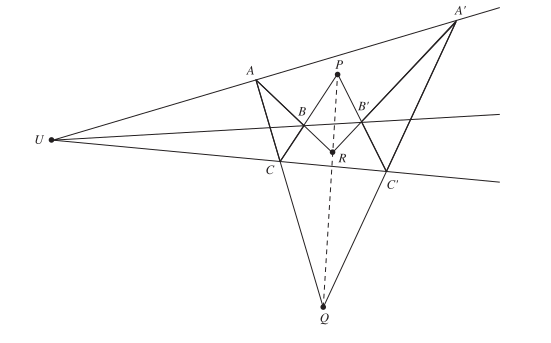
\includegraphics[width=0.75\linewidth]{pictures/desargues.png}
  \caption{Figure from \cite{brannan}.}
\end{figure}

\begin{proof}
  We will prove the theorem for the special case where $A=[1:0:0]$, $B=[0:1:0]$, $C=[0:0:1]$,
  and $U=[1:1:1]$. From the fundamental theorem of projective geometry, we know that it will be
  congruent to any other configuration. We can use the fact that projective congruence preserves
  projrctive properties, to deduce that the theorem holds in general.

  The line $AU$ has the equation $y=z$. Since $A'$ lies on $AU$, it must have coordinates
  $[a:b:b]$, where $b\ne 0$, since $A'\ne A$. We can also wirte $A'=[p:1:1]$, where $p=a/b$.
  Similary, $B'=[1:q:1]$, and $C'=[1:1:r]$.

  Now to find the point $P$, we find the equation of the line $BC$.
  \[
    \begin{vmatrix}
      x & y & z\\
      1 & q & 1\\
      1 & 1 & r
    \end{vmatrix}
    =0\Longrightarrow (qr-1)x-(r-1)y+(1-q)=0
  \]
  Substituting $x=0$ in the equation for the line $B'C'$, we get $(r-1)y=(1-q)z$, which immplies
  $P=[0:1-q:r-1]$. Similarly we find that $Q=[1-p:0:r-1]$, and $R=[1-p:q-1:0]$.

  To check the colinearity of $P$, $Q$, and $R$:
  \[
    \begin{vmatrix}
      0   & 1-q & r-1 \\
      1-p & 0   & r-1\\
      1-p & q-1 & 0
    \end{vmatrix}
  \]
  \begin{eqnarray*}
    &=& -(1-q)(1-p)(1-r)+(r-1)(1-p)(q-1)\\
    &=& 0
  \end{eqnarray*}

  i.e $P$, $Q$, and $R$ are colinear.
\end{proof}

Proof adapted from \cite{brannan}.

\begin{prop}
  There is a unique projective conic through any given set of five points.
\end{prop}

\begin{proof}
\end{proof}

Proof adapted from \cite{brannan}.

\begin{remark}
  \textbf{The Standard Projective Conic}\\
\end{remark}

\begin{prop}
  Let $E_1$ and $E_2$ be non-degenrate conics that pass through the points $P_1$, $Q_1$, $R_1$
  and $P_2$, $Q_2$, $R_2$ respectively. THen ther exists a projective transformation $t$ which
  maps $E_1$ to $E_2$ such that $t(P_1)=P_2$, $t(Q_1)=Q_2$, and $t(R_1)=R_2$.
\end{prop}

Proof adapted from \cite{brannan}.

\begin{theorem}[Pascal's Theorem]
\end{theorem}

\begin{figure}[H]
  \center
  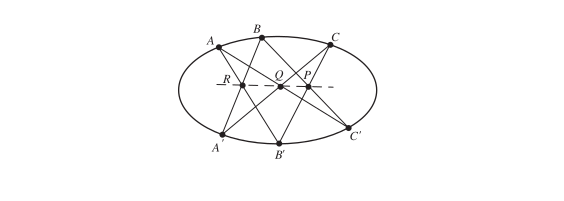
\includegraphics[width=\linewidth]{pictures/pascal.png}
  \caption{Figure from \cite{brannan}.}
  \label{fig:pascal}
\end{figure}

\begin{proof}
\end{proof}

Proof adapted from \cite{brannan}.

\section{The Cross-Ratio}

\begin{definition}
  Let $a$, $b$, $c$ and $d$ be four points on a projective line $D$. There exists a unique map
  from $D$ to $K\cup\{\infty\}$ that maps $a$ to $\infty$, $b$ to $0$, and $c$ to $1$. The
  image of $d$ under this projective mapping is called the \textit{cross-ratio} of the points
  $(a,b,c,d)$, and denoted $[a,b,c,d]$.
\end{definition}

\begin{prop}
  Let $a_1$, $a_2$, $a_3$, and $a_4$ be four points on the line $D$ (the first three being
  distinct) and $a'_1$, $a'_2$, $a'_3$, and $a'_4$ be four points on another line $D'$
  (satisfying the same assumption). There exists a projective transformation $f:D\rightarrow D'$
  such that $f(a_i)=a'_i$ iff $[a_1,a_2,a_3,a_4]=[a'_1,a'_2,a'_3,a'_4]$.
\end{prop}

\begin{proof}
  Assume $f$ is a projective mapping that sends $a_i$ to $a'_i$. Let 
\end{proof}

\section{Elliptic Curves}

\begin{definition}
  An elliptic curve is a non-empty, non-singular, degree 3 projective curve. \cite{spallone}
\end{definition}

\subsection{Group Laws on Conics}


  \bibliographystyle{alpha}
  \bibliography{main}

\end{document}
